\documentclass[sigconf,anonymous]{acmart}

\usepackage{arydshln}
\usepackage{hyperref}
\usepackage{multirow}
% \usepackage[utf-8]{inputenc}
\usepackage{geometry}
\usepackage{listings}
\usepackage{xcolor}
\usepackage{amsmath} 
\usepackage{amsfonts}

\lstdefinelanguage{json}{
    basicstyle=\small\ttfamily,
    numbers=left,
    numberstyle=\tiny,
    stepnumber=1,
    numbersep=8pt,
    showstringspaces=false,
    breaklines=true,
    frame=lines,
    backgroundcolor=\color{gray!10},
    literate=
     *{0}{{{\color{blue}0}}}{1}
      {1}{{{\color{blue}1}}}{1}
      {2}{{{\color{blue}2}}}{1}
      {3}{{{\color{blue}3}}}{1}
      {4}{{{\color{blue}4}}}{1}
      {5}{{{\color{blue}5}}}{1}
      {6}{{{\color{blue}6}}}{1}
      {7}{{{\color{blue}7}}}{1}
      {8}{{{\color{blue}8}}}{1}
      {9}{{{\color{blue}9}}}{1}
      {:}{{{\color{red}{:}}}}{1}
      {,}{{{\color{red}{,}}}}{1}
      {\{}{{{\color{purple}{\{}}}}{1}
      {\}}{{{\color{purple}{\}}}}}{1}
      {[}{{{\color{purple}{[}}}}{1}
      {]}{{{\color{purple}{]}}}}{1},
}

\AtBeginDocument{%
  \providecommand\BibTeX{{%
    Bib\TeX}}}

\setcopyright{acmlicensed}
\copyrightyear{2026}
\acmYear{2026}
\acmDOI{XXXXXXX.XXXXXXX}
%% These commands are for a PROCEEDINGS abstract or paper.
\acmConference[SIGIR '26]{Make sure to enter the correct
  conference title from your rights confirmation email}{July XX--YY,
  2026}{Somewhere, Asia}

\acmISBN{978-1-4503-XXXX-X/2018/06}
\begin{document}

\title{Identifying the most crucial bibliographic research entries in mathematics as recommendations}
% Identifying the most crucial works for research papers in mathematics as recommendations
% an aspect aware CB-RS for largest pure and applied math BREs DB zbMATH open

\author{Ankit Satpute}
\email{Ankit.Satpute@fiz-karlsruhe.de}
\orcid{0000-0003-3219-026X}
\affiliation{
  \institution{FIZ Karlsruhe Leibniz Institute for Information Infrastructure}
  \streetaddress{Franklinstrasse 11}
  \city{Berlin}
  \country{Germany}
  \postcode{10587}
}

\author{Noah Gießing}
\email{Noah.Giessing@fiz-karlsruhe.de}
\orcid{0009-0006-5268-2519}
\affiliation{
  \institution{FIZ Karlsruhe Leibniz Institute for Information Infrastructure}
  \streetaddress{Franklinstrasse 11}
  \city{Berlin}
  \country{Germany}
  \postcode{10587}
}

\author{Andr\'{e} Greiner-Petter}
\email{Greiner-Petter@gipplab.org}
\orcid{0000-0002-5828-5497}
\affiliation{
  \institution{George August University of Göttingen}
  \streetaddress{Wilhelmsplatz 1}
  \city{Göttingen}
  \country{Germany}
  \postcode{37073}
}

\author{Moritz Schubotz}
\email{Moritz.Schubotz@fiz-karlsruhe.de}
\orcid{0000-0001-7141-4997}
\affiliation{
  \institution{FIZ Karlsruhe Leibniz Institute for Information Infrastructure}
\streetaddress{Franklinstrasse 11}
  \city{Berlin}
  \country{Germany}
  \postcode{10587}
}

\author{Olaf Teschke}
\email{Olaf.Teschke@fiz-karlsruhe.de}
\orcid{0009-0003-4089-9647}
\affiliation{
  \institution{FIZ Karlsruhe Leibniz Institute for Information Infrastructure}
  \streetaddress{Franklinstrasse 11}
  \city{Berlin}
  \country{Germany}
  \postcode{10587}
}

\author{Akiko Aizawa}
\email{aizawa@nii.ac.jp}
\orcid{0000-0001-6544-5076}
\affiliation{
  \institution{National Institute of Informatics}
  \streetaddress{2 Chome-1-2 Hitotsubashi}
  \city{Tokyo}
  \country{Japan}
  \postcode{101-0003}
}

\author{Bela Gipp}
\email{gipp@uni-goettingen.de}
\orcid{0000-0001-6522-3019}
\affiliation{
  \institution{George August University of Göttingen}
  \streetaddress{Wilhelmsplatz 1}
  \city{Göttingen}
  \country{Germany}
  \postcode{37073}
}

\renewcommand{\shortauthors}{Satpute et al.}

\begin{abstract}
Mathematical research papers differ from those in most other scientific domains: their connections are often conceptual, structural, or logical rather than lexical or empirical. 
Existing recommender systems for research papers typically rely on textual or citation-based similarity, which may not capture mathematics specific relationships. 
In this paper, we investigate what recommendations in mathematics look like and establish the first two datasets of mathematical paper recommendations, GoldRiM and SilverRiM, capturing concrete ways in which mathematical research papers are related and could be recommended. 
GoldRiM is a small, high-quality, expert-annotated dataset of 420 recommendations, capturing seven distinct conceptual relationship types. 
SilverRiM is a large-scale, automatically generated dataset of 919K recommendation pairs and 7,241 aspects, extracted using LLM-based aspect identification from 812K zbMATH reviews. 
Together, they reveal that mathematical recommendations are driven by aspect-level conceptual relationships, such as extension, specialization, or motivation, rather than surface-level textual similarity. 
We release both datasets publicly to facilitate future research on mathematics-aware recommendation systems and conceptual similarity modeling.
\end{abstract}

\begin{CCSXML}
<ccs2012>
 <concept>  <concept_id>00000000.0000000.0000000</concept_id>
  <concept_desc>Do Not Use This Code, Generate the Correct Terms for Your Paper</concept_desc>
  <concept_significance>500</concept_significance>
 </concept>
 <concept>
  <concept_id>00000000.00000000.00000000</concept_id>
  <concept_desc>Do Not Use This Code, Generate the Correct Terms for Your Paper</concept_desc>
  <concept_significance>300</concept_significance>
 </concept>
 <concept>
  <concept_id>00000000.00000000.00000000</concept_id>
  <concept_desc>Do Not Use This Code, Generate the Correct Terms for Your Paper</concept_desc>
  <concept_significance>100</concept_significance>
 </concept>
 <concept>
  <concept_id>00000000.00000000.00000000</concept_id>
  <concept_desc>Do Not Use This Code, Generate the Correct Terms for Your Paper</concept_desc>
  <concept_significance>100</concept_significance>
 </concept>
</ccs2012>
\end{CCSXML}

\ccsdesc[500]{Do Not Use This Code~Generate the Correct Terms for Your Paper}
\ccsdesc[300]{Do Not Use This Code~Generate the Correct Terms for Your Paper}
\ccsdesc{Do Not Use This Code~Generate the Correct Terms for Your Paper}
\ccsdesc[100]{Do Not Use This Code~Generate the Correct Terms for Your Paper}


\keywords{}

\received{20 February 2007}
\received[revised]{12 March 2009}
\received[accepted]{5 June 2009}

%%
%% This command processes the author and affiliation and title
%% information and builds the first part of the formatted document.
\maketitle

\section{Introduction}
% A content-based research paper recommender system recommends papers that are similar in content. 
% However, similarity is an ill-defined concept as research paper articles might be similar in many aspects, such as using the same concept, the same previous work, the same tools, etc.
% While existing ABRPRS have considered different aspects to bring recommendations, none of them consider aspects in research papers from pure and applied mathematics.
% Research papers from pure and applied mathematics are different than a typical computer science research paper where we have abstract, introdction, related work section, etc, on the other hand in math we ususally dont have such a structure as papers often just start with two sentence abstract and give the proof, alternate proof, analyze acse extension of previuso proof etc. 
% There doesnt exists any data that is seggregated in terms of sections or analysis on the doucment level. 
% As a proof of concept we created a small dataset of research papers in pure and pplied mathmetaics ad their most important ocnnection using an expert. 
% While we argue that the data is small and might miss sme connections but just to check how the connection in papers looks llike a is a goo start. 
% We then analyzed the connections to categorieze how these paper might be connected. 
% Figure 1 shows a papaer and their conenctions.
% These are fundamentally differrent from the connection in existing dataset. 
% Idntifying such cnnection adds up a difficutly if there are no full-texts availabel which is the cas ein bibliographic digital librares such as zbMATh open. 

% While existing aspects provide information on how they are similar, they are still on a broad level of similarity.
% Aspects such as introduction, Related work, dataset, etc., are helpful in general similarity; however, they don't provide insight into exactly how these datasets are connected to the paper.
% In mathematics, datasets are not commonly used, especially in pure and applied mathematics research.
% There exists a citation intent or aspect, such as positive, negative, or neutral, but it does not indicate how it is utilized.

% % To understand how research papers in mathematics might be connected we created a 

% Domain specific bibliographic digital research paper libraries have been a primary source for exploration in many domains, where people go at first to explore connections between articles. 
% Example for such are DBLP (for computer science), PubMed (medicine), zbMATH Open (mathematics), etc.
% None of such libraries currently have a recommender system to suggest articles that might be connected to the article currently viewed by a user. 


% \section{Related work}

% Related work in three categories.
% Aspect-based similarity in research papers by text content
% Citation-intent prediction or classification.
% GNN for link prediction and ranking, enabling the discovery of new connections.

\section{RQ1: What do recommendations in mathematics look like?}

% Bullet points summarry: 
% 1. We ask a mathematician to give us recommendations (so we create GoldRiM).
% 2. We checked how similar to get unique connections.
% 3. They are indeed connected in more theorotical or extsnion way. (also explain why it is difficult to get that vased on BREs bcz BRES are very specific the doent have full text and even with full text it could be difficult as it doesnt follow the same structure)
% 4. Are such recommendations also vailable in other domain, yes, but they have broad categories ours (maths) are more distinct.
% 5. Existiing work get these aspects through citation mentions, good to have bulk data.
% 6. We dont have full appers as math appers dont really have section wise thing or there is no other dataset availabel to do so.
% 7. We go to reviews as gives us indication on how in-review citations are similar.
% 8. We see what is overlapping or differrent in both datasets.
% 9. They can be used compliemnetary depending on the scale.
% 10. How does it compare with other datasets?
In this research question, we investigate how recommendations in mathematics could be and establish two datasets.
To the best of our knowledge, no prior dataset of research paper recommendations in mathematics exists.
We therefore collaborated with an expert mathematician to manually provide recommendations and analyze their nature.
This results in a small, high-quality \textbf{Gold}-standard dataset of \textbf{R}ecommendations \textbf{i}n \textbf{M}athematics (\textbf{GoldRiM}).
Motivated by the insights from \textbf{GoldRiM}, we subsequently developed a large-scale, automatically constructed \textbf{Silver}-standard dataset of \textbf{R}ecommendations \textbf{i}n \textbf{M}athematics (\textbf{SilverRiM}).
Both datasets are derived from zbMATH Open\footnote{\url{https://zbmath.org/}}, one of the most comprehensive digital libraries in pure and applied mathematics~\cite{deb2024zbmathovrvw}.
In the following sections, we first introduce zbMATH Open and then describe how \textbf{GoldRiM} and \textbf{SilverRiM} were created, highlighting what they reveal about the nature of mathematical recommendations.

\subsection{zbMATH Open}
We utilize zbMATH Open and their reviewers to study recommendations in mathematics.
zbMATH open contains Bibliographic Research Entries (BREs), which contain research metadata such as title, keywords, Mathematics Subject Classification codes, authors, year, and more.
zbMATH Open BREs contains one of the following: a review, a summary, both of which are written by reviewers, or an abstract of the research paper.
Full texts are not included, but zbMATH Open provides links to publishers or repositories where they can be accessed.
Reviewers in zbMATH Open are experts in mathematics who provide a review or summary (hereafter referred to as a review), a well-balanced description of the paper's content within the context of current developments in the corresponding subject area. 
They are trained mathematicians who are selected by the editor-in-chief of zbMATH Open, based on their publication record, teaching experience, and overall expertise in the field.
Thus, zbMATH Open reviews provide rich, expert-written context for understanding how a paper conceptually connects to others, making it ideal for studying recommendation relationships.

\subsection{GoldRiM}
We first collaborated with an experienced zbMATH Open reviewer to manually construct the \textbf{GoldRiM} dataset.
The reviewer was given 80 randomly selected BREs (seeds) from their area of expertise and asked to recommend content-wise similar BREs, i.e., papers they would naturally read next.
This process yielded 420 recommendations for the 80 seed papers.
To analyze why these particular recommendations were chosen, we first examined simple overlaps in text, mathematical expressions, and citations.
We found that the textual and mathematical overlap between seeds and recommendations was minimal, often limited to a few shared terms or symbols.
Additionally, about 47\% of recommendations involved direct citation links (either the seed cited the recommendation or vice versa), but many other cited papers were not recommended.
The remaining 53\% of pairs had no citation overlap at all.
Hence, surface-level similarity in text, formula, or citation was insufficient to explain the expert’s recommendations.

We therefore conducted a qualitative analysis on 100 seed-recommendation pairs (across 27 seeds).
For each pair, we examined metadata, reviews, and, where available, full texts, to infer why a recommendation was made.
When citations existed, we tried to find why this particular citation was made and not others by looking at full texts or what the contribution of an article was over its cited one.
For non-cited pairs, we consulted the expert reviewer to understand the conceptual connection.
This analysis revealed diverse kinds of relationships, each representing a specific aspect of similarity.
We merged them into seven categories, summarized in Table~\ref{tab:goldrim_aspects}.
For example, the category \textit{Extend}, assigned where one paper extends the ideas, methods, or proofs of another.
% This extension, however, if it cites the paper it extends, the citation occurs only a few times and sometimes even once, where authors simply mention it in the full-text and proceed with the proof or further analysis.
% There were other papers that also extend the seed, but the recommendation is given because this extension is more influential and reveals important things than other extensions. This was explained by the reviewer.
% In some cases, the seed extends the recommendation and is not cited because citation info is not available in zbMATH Open, but in the full-texts only.
% One other example is the category \textit{Alternativ}, in which the seed provides an alternative approach to what is done in the recommendation. 
% There might be other alternative approaches, but this approach by seed uncovers something crucial in math that is surprising or not expected.
These categories capture how recommendations were related, not by textual similarity, but by logical, conceptual, or structural connections.
For instance, a paper may extend another’s theorem without extensive textual overlap or even direct citation, yet experts perceive them as inherently linked.
In summary, \textbf{GoldRiM} provides the first evidence that recommendations in mathematics are driven by aspect-level conceptual relationships, rather than surface features.
The dataset (and its construction pipeline) is publicly available\textsuperscript{\ref{gitlink}}.
While limited in scale and based on a single expert, it provides a foundational understanding of what “recommendation” means in the mathematical domain.
It is possible that other experts or similar connected papers might reveal different aspects and provide more insights into how recommendations in mathematics are presented.
This motivates us to look for such recommendations at scale.

% A brief description of each of the seven aspects is provided in Table~\ref{tab:goldrim_aspects}.
% The identified aspects tell us that mathematical recommendations could be connected based on theoretical and concrete connections that might not be visible by just bibliographic info or full-text overlap but one might need to have a deep understanding of the concepts to know hey they are connected or can be obtained on deep foundational level on how they are connected.
% We observed from annotation of categories that the connection between recommendations is more logical, conceptual, or structural than mere overlap of tokens or citation sharing in view of content similarity.  
% In this section, we created \textbf{GoldRiM}, the first dataset of recommendation mathematics and tried to discover how recommendations in mathematics look like. 
% The Dataset and its construction steps are freely available\textsuperscript{\ref{gitlink}}.
% However, the resulting dataset is small and we only used one expert to obtain recommendations and identify aspects. 

\subsection{SilverRiM}

\begin{figure}
    \centering
    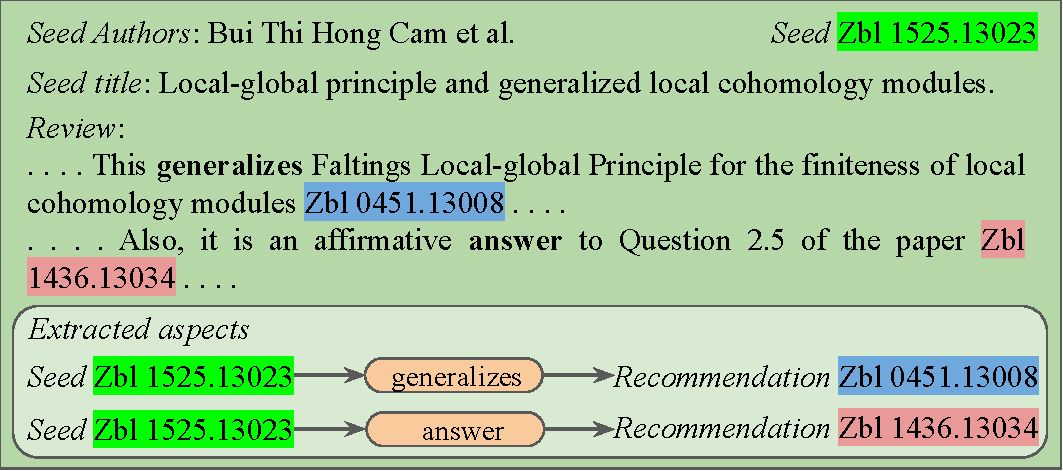
\includegraphics[width=0.48\textwidth]{images/aspect_SILVERst.pdf}
    \caption[An example seed BRE from zbMATH Open]{%
        An example seed BRE (Zbl 1525.13023~\cite{exSeedBRE})\protect\footnotemark[1]
        from zbMATH Open with potential recommendations 
        (Zbl 0451.13008\protect\footnotemark[2]~\cite{exRecmndBRE1}, 
        Zbl 1436.13034\protect\footnotemark[3]~\cite{exRecmndBRE2}) and extracted aspects 
        in the SilverRIM dataset.%
    }
    \label{fig:exampleSILVER}
\end{figure}
\footnotetext[1]{\url{https://zbmath.org/1525.13023}}
\footnotetext[2]{\url{https://zbmath.org/0451.13008}}
\footnotetext[3]{\url{https://zbmath.org/1436.13034}}

In zbMATH Open, reviewers often cite other works directly within the review texts they write (in-review citations).
A reviewer may cite a prior paper to highlight an important connection in a method, a shared motivation, or a result, among other reasons.
We consider these in-review citations as weak signals for recommendations.
Since recommendations in \textbf{GoldRiM} also show strong citation overlap, it is reasonable to treat in-review citations as recommendations.
When the cited works exist in zbMATH Open, reviewers include the respective ID (Zbl) to enable direct access.
These in-review citations, along with the sentences in which they appear, reveal the relationship between the citing and cited works, similar to the aspects identified in \textbf{GoldRiM}.
This helps us uncover additional aspects through which recommendations in mathematics may be related.
Figure~\ref{fig:exampleSILVER} shows an example zbMATH Open seed BRE with its in-review citations as potential recommendations.
The two aspects, \textit{generalizes} and \textit{answer}, in the example indicate distinct relationships between the recommendations and the seed paper.

As of October 2025, zbMATH Open contains 812,241 BREs with 1,286,410 in-review citations.
Manual extraction of in-review citations and their aspects across millions of BREs is infeasible.
Considering that obtaining a single review in zbMATH Open already requires several months\footnote{\url{https://zbmath.org/about/\#:~:text=Indexing\%20decisions\%22.-,Reviewing,-Published\%20items\%20are}}.
We expect a similar amount of time for manually constructing recommendations and aspects, as both require comparable expertise.
Therefore, we employ an LLM-based approach to automatically extract such relationships.
To obtain aspects, we utilize Qwen2.5-14B~\cite{qwen2025qwen25technicalreport} as it's the best-performing~\cite{koloveas2025can} few-shot model in the citation-intent prediction task on the SciCite~\cite{cohan2019structural} and ACL-LRC~\cite{Jurgens2018ACLARC} datasets.
On both datasets, Qwen2.5-14B was able to identify the relationship, such as \textit{Background}, \textit{Method}, or \textit{Result}, in which research papers are similar, with the highest accuracy among instruction LLMs.
Although LLM-based extractions are not as accurate as humans, annotations with prompts such as phrase extraction produce human-annotated-like data if not better than humans~\cite{horych-etal-2025-promises,tan-etal-2024-large}.
Our objective here is not to evaluate the LLM, but to leverage it to efficiently generate weakly supervised relationships to understand how recommendations in mathematics are connected.
This allows us to construct a large-scale dataset with aspect-level explanations for recommendations.

We designed a concise few-shot prompt (Appendix~\ref{Appendix:prompt}) with three examples, as prior work indicates that larger prompts (e.g., 10 examples) reduce accuracy~\cite{koloveas2025can}. 
The model is asked to relationship in JSON format, enabling structured outputs even when multiple citations appear within a single review.
We passed 812,241 BREs through Qwen2.5-14B using the designed prompt and asked it to get the mentioned Zbl citation along with the aspect.
It worked correctly for 795,871 BREs, and for others, it gave either erroneous JSON, no aspect, or an invalid Zbl.  
It assigned 978,238 unique relationships (including stop words) as a different aspect\footnote{counted considering \textit{Extends} and \textit{Extends to} as a separate relationship.}) for 1,031,239 BRE pairs.
We apply the following quality check steps to obtain the final set of aspects.
First, \textbf{Normalization}, in which we stem and lemmatize extracted aspects using the Porter Stemmer, reducing them to a consistent set of 10,728 base forms.
For example, \textit{introduce}, \textit{introduced}, \textit{introduces}, \textit{introducing} becomes \textit{introduce}.
Second, \textbf{Filtering}, we manually inspected the normalized relationships having less than 1000 BREs to remove those that did not make sense due to probable LLM errors or absence of a potential single-word aspect in the review. 
Such relationships include \textit{due}, \textit{first}, \textit{conference}, \textit{see}, \textit{roll}, etc. 
This step yields 919,655 recommendations with 7,241 aspects for 745,264 BREs.

The top 20 aspects and their frequencies are shown in Figure~\ref{fig:SilverRIMwordFreq}, and their short description devised based on examples is in Appendix Table~\ref{tab:silverrim_aspects}.
The aspect with the most BREs, i.e., \textit{collect} represents\footnote{For example, \url{https://zbmath.org/1557.90300} mentions a reference to a conference collection \url{https://zbmath.org/1531.93014} at zbMATH Open.} a collection of lecture notes or conference proceedings, such as an entry at zbMATH Open.
The aspects are shared across many papers, which shows that common patterns of connections exist in recommendations.
Four of the \textbf{GoldRiM} aspects: \textit{Motiv}, \textit{Case}, \textit{Extend}, and \textit{Compare} also appear in \textbf{SilverRiM}, confirming the reliability of the LLM-based aspects extraction.
Three aspects: \textit{Applic}, \textit{Alternativ}, and \textit{Specialize} are unique to \textbf{GoldRiM}, suggesting finer-grained distinctions made by the expert reviewer that were not captured in \textbf{SilverRiM}.
However, these distinctions are related to similar categories in \textbf{SilverRiM}.
For example, the \textit{Alternativ} aspect in \textbf{GoldRiM}, which captures relationships between studies offering alternative approaches, is conceptually close to the \textit{studi} aspect in \textbf{SilverRiM}, where the reviewer expresses it as “study.”
We retain these distinctions for future qualitative analyses, as they may be useful in differentiating types of similarity. 
The additional aspects identified in \textbf{SilverRiM} confirm our understanding from \textbf{GoldRiM} that mathematical recommendations are connected through distinct aspects.
Moreover, they expand the number of identified aspects, revealing additional discrete ways in which recommendations are connected—through theoretical, logical, and conceptual relationships rather than simple textual or formulaic similarity.
These relationships allow us to model recommendations as being linked through multiple types of aspects.
Dataset characteristics are summarized in Table~\ref{tab:dataset_characteristics}, and the construction steps are freely available\footnote{\url{https://anonymous.4open.science/r/Aspect-Similarity-Math-BRE-Recsys-8098/}\label{gitlink}}. 

\begin{figure}
    \centering
    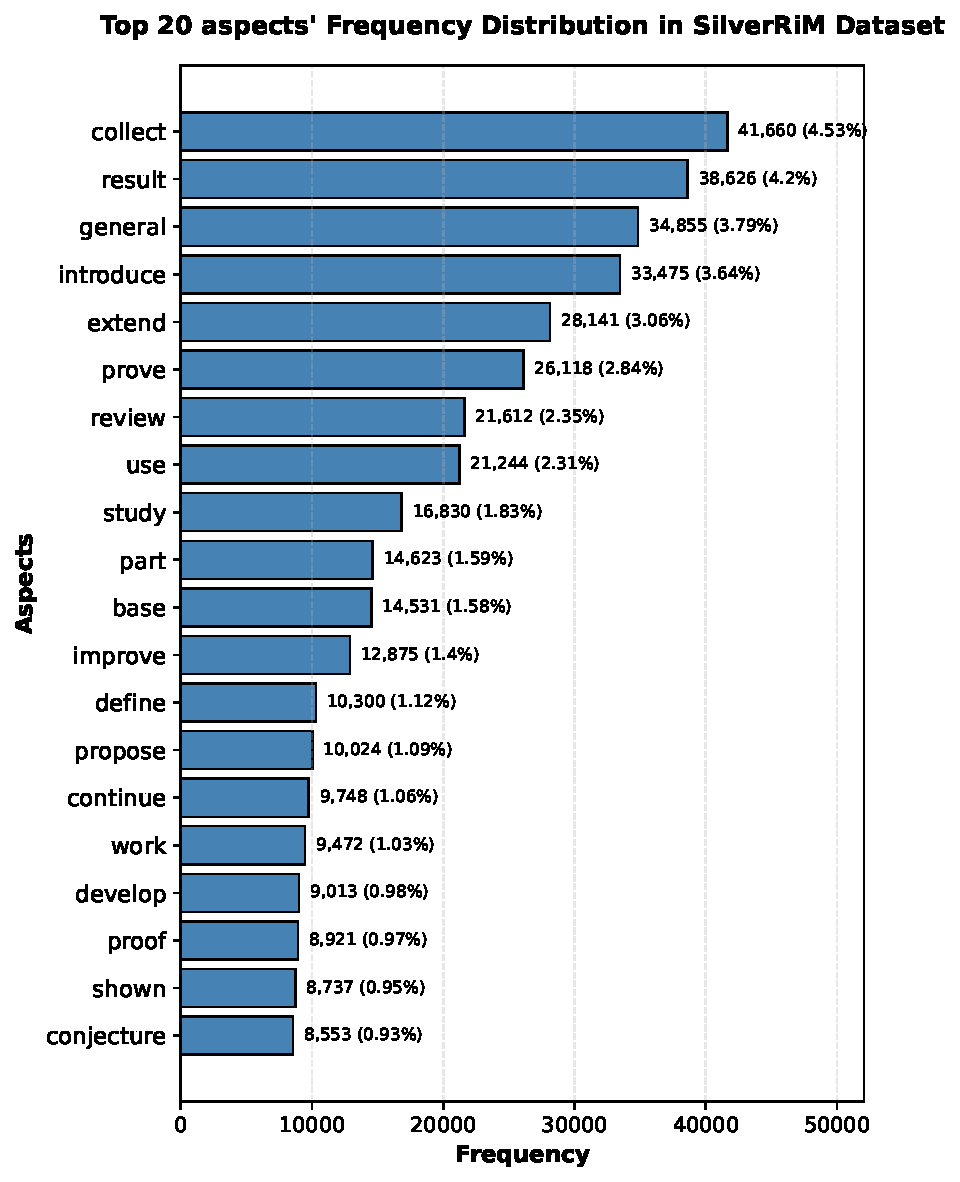
\includegraphics[width=0.5\textwidth]{images/silverrim_aspect_frequency_combined_halfway.pdf}
    \caption{Top 20 aspects' frequency distribution in the SilverRiM dataset.}
    \label{fig:SilverRIMwordFreq}
\end{figure}

\begin{table}[h]
\centering
\caption{Characteristics of GoldRiM and SilverRiM Datasets}
\label{tab:dataset_characteristics}
\begin{tabular}{lcc}
\hline
\textbf{Characteristic} & \textbf{GoldRIM} & \textbf{SilverRIM} \\
\hline
Total BRE Seeds & 80 & 745,264 \\
BRE Pairs (Recommendations) & 420 & 919,655 \\
Unique aspects & 7(100 pairs) & 7,241 \\
Recommendations per Seed & 5.25 & 1.23 \\
\hline
\end{tabular}
\end{table}

\subsection{RQ1 discussion}

\begin{table*}[h]
\centering
\caption{Categorizations of aspects in previous works vs our curated math-specific work.}
\label{tab:aspects}
\begin{tabular}{lll}
\hline
Dataset & Categorization of aspects & \# of doc pairs\\
%add lable extraction manual or artificial using tools?
\hline
Modified AAN~\cite{chakraborty2016ferosa} & Background, Alternative Approaches, Methods, Comparison & 61,051\\
PICO~\cite{jain2018PICObiomed} & Population, Interventions, Outcomes & 41,000\\
CSCW~\cite{chan2018solventCSCW} & Background, Purpose, Mechanism, Findings & 1225\\
Papers with code~\cite{Ostendorff2022a} & Task, Dataset, Result & 1,570,235\\
Modified ACL~\cite{kobayashi2018ACL} & Objective, Method, Result & 34,760\\
ACL-ARC~\cite{Jurgens2018ACLARC} & Background, Method, Result & 1,941\\
SciCite~\cite{cohan2019structural} & Background, Method, Result & 11,020\\
\hline
GoldRiM (Ours)& Extend, Case, Applic, Alternativ, Motiv, Specialize, Compare & 7,241\\
SilverRiM (Ours)& Collec, Result,  Gener, Introduc, Extend, prove, review, and 7,232 other & 89,786\\
\hline
\end{tabular}
\end{table*}

To address RQ1, we established the \textbf{GoldRiM} and \textbf{SilverRiM} datasets, demonstrating that recommendations in mathematics are connected by aspect-level conceptual relationships rather than surface-level similarity.
Furthermore, identifying such aspects is difficult to judge based on the surface information available in zbMATH Open; one must understand their conceptual relationships or consult the full text, which might not be available for many zbMATH Open BREs.
Aspect-based similarity of research papers for recommendation has been studied before~\cite{Ostendorff2022a,chakraborty2016ferosa,cohan2019structural}.
However, such studies have not focused on mathematical aspects, but rather on fields like computer science, biomedical research, and mixed-domain research papers, often excluding mathematics papers.
In Table~\ref{tab:aspects}, we compare our identified and established mathematics-specific aspects with those used in previous studies on aspect-based similarity for recommendations.
There are several shared aspects between our work and existing studies, including \textit{Results}, \textit{Alternative Approaches}, and \textit{Comparisons}.
Some aspects may appear synonymous, for example, (\textit{Background} in existing work vs. \textit{Compare} in ours), but they differ in what each aspect represents and its underlying purpose.
First, existing datasets primarily include broad categories typically derived from the sections of research papers where citations are found.
However, such section-based aspects only provide a rough indication of research article similarity.
They do not capture the actual reason or aspect behind the connection, whether the cited work is mentioned for context, used as a method, extended, compared, improved upon, or otherwise.
In contrast, our aspects indicate whether a cited work is actually being used or relied upon, as interpreted by expert reviewers in mathematics.
For example, our aspect \textit{Alternative Approach} refers to an alternative proof, analysis, or conjecture presented in a research paper, while in existing datasets, the corresponding aspect generally includes all related work mentions without specifying which one is directly applicable.
Second, the aspects in \textbf{SilverRiM} and \textbf{GoldRiM} capture mathematics-specific conceptual relationships that are not present in existing datasets.
For example, aspects such as \textit{Generalization}, \textit{Conjecture}, \textit{Theorem}, and \textit{Construct}, among others, identified in our datasets, are unique to mathematics and not present in previous studies.
This allows us to identify 7,241 distinct aspects, scale enabled by the reviews in zbMATH Open.

In summary, mathematics-based aspects are more specific, domain-dependent, and explanatory than section-based aspects seen in existing datasets.
This distinction highlights that mathematical research relationships are defined less by empirical evidence or datasets and more by logical, structural, and conceptual reasoning across problems, proofs, and methods.
These findings directly address RQ1, demonstrating that recommendations in mathematics are based on aspect similarity, which differs from the aspects observed in other research domains.
The identified aspects reveal that mathematical works are connected through theoretical development and conceptual relationships unique to the discipline, unlike those represented in existing datasets.
This domain-specific nature underscores the importance of our newly established datasets for advancing recommendations in mathematics.

\section{RQ2: How do existing systems perform? and qualitative analysis}

doc1, doc2, aspectlabel 0 or 1, train model for each aspect, and then get similar candidates for each aspect by retrieving embeddings.
For each aspect you need to train an embedding model, so it is infeasible to have 560 embedding models, with each model having to embed 5 million docs for retrieval. 

\section{RQ3: trained GNN for reviewer-preferences based recommendations and qualitative analysis}

\section{Acknowledgments}

We used AI models such as chatGPT, Claude, Perplexity AI to proofread, improve grammar and snetence clarity. EVery sentence in the resulting text is checked by the authors and citations are provided wherever available. We take full responsibility of the texts and results in this manuscript.
%%
%% The next two lines define the bibliography style to be used, and
%% the bibliography file.
\bibliographystyle{ACM-Reference-Format}
\bibliography{main_}


\appendix

\section{Prompt used for extracting SilverRIM aspects}\label{Appendix:prompt}

\section*{Task Description}
You are tasked with extracting the relationship between a statement and its cited work (indicated by a Zbl reference number). Identify the key phrase that describes how the current work relates to each cited work.

Return your answer as a valid JSON object with the following structure:

\begin{lstlisting}[language=json]
{
  "citations": [
    {
      "zbl_number": "the Zbl reference number",
      "relationship": "the key phrase"
    }
  ]
}
\end{lstlisting}

\section*{Examples}

\subsection*{Example 1}

\textbf{Input:} ``For any integral arrangement $U$ and a chamber $\Delta$ the author constructs a local residue form $\omega_\Delta(U)$ and a pairing $\langle,\rangle$ such that for any $t\in\Delta$ one has $B_\Delta f(t)=\langle\omega_\Delta(U),f\exp(t)\rangle$. His constructions are essentially based on the notion of iterated residue of $U_C$-meromorphic functions where $U_C$ is the complexification of the arrangement $U$. The author underlines that his study of these sums was inspired by the works of E. Witten [Commun. Math. Phys. 141, 153-209 (1991; Zbl 0762.53063) and J. Geom. Phys. 9, 303-368 (1992; Zbl 0768.53042)].''

\textbf{Output:}
\begin{lstlisting}[language=json]
{
  "citations": [
    {
      "zbl_number": "Zbl 0762.53063",
      "relationship": "inspired"
    },
    {
      "zbl_number": "Zbl 0768.53042",
      "relationship": "inspired"
    }
  ]
}
\end{lstlisting}

\subsection*{Example 2}

\textbf{Input:} ``The authors investigates the natural question of the rationality of $f$. Previously, J. J. Duistermaat and W. van der Kallen [Indag. Math., New. Ser. 9, No. 2, 221–231 (1998; Zbl 0916.22007)] proved that if $I_\lambda(f_\sigma,\omega)\in C(\lambda)$ and $f$ is a proper non-constant morphism, then $I_\lambda(f_\sigma,\omega)=0$. Here, a necessary and sufficient condition for $I_\lambda(f_\sigma,\omega)$ to extend to a single-valued holomorphic function on the complement of a finite set in $P^1(\mathbb{C})$ is given. By a result of N. Nilsson [Ark. Mat. 5, 527–540 (1965; Zbl 0144.36302)] this is equivalent to the rationality of $I_\lambda(f_\sigma,\omega)$. Moreover, the criterion can be used to determine the set $\{\sigma\mid I_\lambda(f,\sigma,\omega)\in C(\lambda)\}$ from the pair $(f,\omega/df)$ when $X$ is a curve.''

\textbf{Output:}
\begin{lstlisting}[language=json]
{
  "citations": [
    {
      "zbl_number": "Zbl 0916.22007",
      "relationship": "proved"
    },
    {
      "zbl_number": "Zbl 0144.36302",
      "relationship": "result"
    }
  ]
}
\end{lstlisting}

\subsection*{Example 3}

\textbf{Input:} ``The paper under review was motivated by some questions on compact Lie groups raised by O. Mathieu [in: Algèbre non commutative, groupes quantiques et invariants. Sémin. Congr. 2, 263–279 (1995; Zbl 0889.22008)]. In the last section, the author gives a counterexample to Mathieu's second conjecture.''

\textbf{Output:}
\begin{lstlisting}[language=json]
{
  "citations": [
    {
      "zbl_number": "Zbl 0889.22008",
      "relationship": "motivated"
    }
  ]
}
\end{lstlisting}

\subsection*{Example 4}

\textbf{Input:} ``Now, strictly speaking the second category does not make sense at the present time since the semi-infinite flag manifold does not carry an algebro-geometric structure allowing a theory of perverse sheaves on it. The authors circumvent this problem by defining an ad-hoc category $\text{Perv}(\text{Fl}_{\infty/2})$; this approach was initiated in [M. Finkelberg, I. Mirkovic, Differential topology, infinite-dimensional Lie algebras, and applications. D. B. Fuchs 60th anniversary collection. Providence, RI: American Mathematical Society. Transl., Ser. 2, Am. Math. Soc. 194(44), 81–112 (1999; Zbl 1076.14512)]. The definition uses a geometric object introduced by Drinfeld and denoted $\overline{\text{Bun}}_{N^-}$. This object $\overline{\text{Bun}}_{N^-}$ classifies principal $G$-bundles on $X$ endowed with a possibly degenerate reduction to the maximal unipotent subgroup $N^-$; see [A. Braverman, M. Sanz-Solé, (ed.) et al., Proceedings of the international congress of mathematicians (ICM), Madrid, Spain, August 22–30, 2006. Volume II: Invited lectures. Zürich: European Mathematical Society (EMS), 1145–1170 (2006; Zbl 1118.22007)] for more details and references.''

\textbf{Output:}
\begin{lstlisting}[language=json]
{
  "citations": [
    {
      "zbl_number": "Zbl 1076.14512",
      "relationship": "initiated"
    },
    {
      "zbl_number": "Zbl 1118.22007",
      "relationship": "details"
    }
  ]
}
\end{lstlisting}

\section*{Test Case}

\textbf{Input:} ``About fifteen years ago, the physicist E. Verlinde proposed a stunning formula for the dimension of the space of conformal blocks within the Wess-Zumino-Witten model of conformal quantum field theory. Verlinde's formula involves certain rational trigonometric sums of highly complicated combinatorial structure, whose effective computation represents a real mathematical challenge. On the other hand, this formula turned out to have a close relationship to the geometry of the moduli spaces of flat connections over compact Riemann surfaces, and it was this spectacular, utmost striking discovery that opened the way to computing various intersection numbers in the enumerative geometry of such moduli spaces. The paper under review makes another step forward in this direction. Namely, in order to help to uncover the geometric information hidden in Verlinde's formula, the author derives a compact polynomial formula computing certain rational trigonometric sums occuring in this context. Building upon his earlier results on rational sums and Bernoulli polynomials corresponding to central hyperplane arrangements [A. Szenes, Int. Math. Res. Not. 1998, No. 18, 937-956 (1998; Zbl 0968.11015)], the author extends these investigations to affine hyperplane arrangements, obtains then a local formula for rational trigonomteric sums of ``Verlinde-type'', and compares his formula to a related result in the work of J.-M. Bismut and F. Labourie [Symplectic geometry and the Verlinde formulas, Surv. Differ. Geom., Suppl. J. Differ. Geom. 5, 97–311 (1999; Zbl 0997.53066)]. In fact, and as the author points out, one of the main goals of his paper under review is to prove the equality of the two formulas, which is achieved in great generality. Finally, the author's local sum formula is also related to the results of M. Brion and M. Vergne on vector partition functions [J. Am. Math. Soc. 10, 797–833 (1997; Zbl 0926.52016)]. However, this particular relationship is still in the process of closer inspection [A. Szenes and M. Vergne, Adv. Appl. Math. 30, 295–342 (2003; Zbl 1067.52014)]. No doubt, the paper under review is an important contribution to the current research on the combinatorics and geometry of the Verlinde formulas.''

\textbf{Expected Output:}
\begin{lstlisting}[language=json]
{
  "citations": [
    {
      "zbl_number": "Zbl 0968.11015",
      "relationship": "results"
    },
    {
      "zbl_number": "Zbl 0997.53066",
      "relationship": "compares"
    },
    {
      "zbl_number": "Zbl 0926.52016",
      "relationship": "related"
    },
    {
      "zbl_number": "Zbl 1067.52014",
      "relationship": "inspection"
    }
  ]
}
\end{lstlisting}

% Appendix: Aspect Definitions
\section*{Appendix A: Aspect Definitions}
\label{Appendix:aspects}

\begin{table*}[h]
\centering
\caption{GoldRiM Aspect Definitions}
\label{tab:goldrim_aspects}
\small
\begin{tabular}{p{2.5cm}p{12cm}}
\hline
\textbf{Aspect} & \textbf{Description} \\
\hline
Extend & extends results, theorems, or methods from the referenced paper to broader contexts, higher dimensions, or more general settings \\
\hline
Case & examines a specific case, special instance, or particular example of concepts presented \\
\hline
Applic & applies methods, theorems, or techniques from the seed paper to solve problems in different mathematical areas or practical domains \\
\hline
Alternativ & presents an alternative approach, different proof method, or competing technique for addressing the same mathematical problem or question \\
\hline
Motiv & provides motivation, context, or foundational ideas that inspired or led to the work \\
\hline
Specialize & focuses on a more specialized or restricted version of the general framework presented \\
\hline
Compare & compares, contrasts, or evaluates different methods, results, or approaches discussed in the seed paper \\
\hline
\end{tabular}
\end{table*}

\begin{table*}[h]
\centering
\caption{SilverRiM Top 20 Aspect Definitions}
\label{tab:silverrim_aspects}
\small
\begin{tabular}{p{2.5cm}p{12cm}}
\hline
\textbf{Aspect} & \textbf{Description} \\
\hline
introduc & used concepts, definitions, objects, or frameworks that are introduced \\
\hline
gener & generalizes results, methods, or structures from more specific or restrictive cases \\
\hline
extend & extends prior results, theorems, or techniques to new settings, dimensions, or conditions \\
\hline
prove & proves theorems, lemmas, or conjectures that are cited or built upon \\
\hline
studi & studies, investigates, or analyzes mathematical objects, phenomena, or structures \\
\hline
part & forms part of a series, related body of work, part 1 or two of the same works or larger research program \\
\hline
propos & proposes new methods, algorithms, conjectures, or theoretical frameworks based on referenced paper \\
\hline
continu & continues research, extends earlier work, or builds upon previous investigations \\
\hline
improv & improves existing results, bounds, estimates, or methods \\
\hline
discuss & discusses topics, questions, or implications that are also addressed in the referenced paper \\
\hline
defin & refrenced papers defines mathematical objects, structures, or concepts that are used in the seed paper \\
\hline
develop & develops theory, methods, or tools that are applied or mentioned \\
\hline
deriv & derives formulas, equations, identities, or results that appear in or relate \\
\hline
correct & corrects errors, refines arguments, or addresses issues from earlier work discussed in the seed paper \\
\hline
investig & investigates properties, behaviors, or characteristics of mathematical structures also studied in the seed paper \\
\hline
conjectur & poses conjectures, open problems, or questions that are addressed or mentioned \\
\hline
translat & translates concepts, results, or methods between different mathematical languages, frameworks, or areas of study \\
\hline
origin & presents original work that serves as a foundation or starting point for developments \\
\hline
question & raises questions, problems, or research directions that are explored or answered \\
\hline
establish & establishes fundamental results, frameworks, or theories that underpin work presented \\
\hline
\end{tabular}
\end{table*}

\noindent \textbf{Note:} These aspect definitions were derived from analysis of in-review citations in zbMATH Open reviews. Aspects describe the relationship between a seed paper and its recommended related work, indicating why the recommendation is relevant to readers of the seed paper.

\end{document}
\endinput
%%
%% End of file `sample-sigconf.tex'.
